\documentclass[a4paper,11pt,oneside]{book}

\usepackage{graphicx}			% to set the title_page image (university's logo)
\usepackage{amsmath} 			% to use the math environments align, aligned, gather, gathered, multline
\usepackage[titletoc]{appendix}
\usepackage{cite}				% to use bibliography
\usepackage{hyperref}			% to use urls
\usepackage{tikz}				% to use flowchart
\usepackage{color, colortbl} 	% to use colors in tables
\usepackage{algorithm2e}		% to insert algorithms
\usepackage{minted}				% for gherkin code in latex
\usepackage{braket}				% to use \Set
\usepackage{subcaption}			% to align two figures in horizontal
\usepackage{synttree}			% for syntaxt-tree

% Defined commands and tools

\newcommand\chap[1]{
  \chapter*{#1}
  \addcontentsline{toc}{chapter}{\protect\numberline{}#1}}

\definecolor{LightCyan}{rgb}{0.76, 0.92, 1}		% cyan
\definecolor{kellygreen}{rgb}{0.3, 0.73, 0.09}	% green
\definecolor{ruddy}{rgb}{1.0, 0.0, 0.16}		% red

\author{Roberto Zen}
\title{Gherkin* and Cucumber*: a new test case path approach to testing Ruby on Rails web applications}

\begin{document}

\begin{titlepage}
	\pagestyle{empty}

	\begin{center}
		{\bfseries\Large {\huge U}NIVERSITY OF {\huge T}RENTO}

		\vspace{0.2cm}

		{\large Department of Information Engineering and Computer Science}

		\vspace{0.5cm}

		\begin{center}
			
\includegraphics[width=0.3\textwidth]{img/unitn}
		\end{center}

		\vspace{0.5cm}

		{\Large Degree course in Computer Science}

		\vspace{0.2cm}
		\line(1,0){338}
		\vspace{0.5cm}

		{\Large Final Thesis}

		\vspace{2.0cm}

		{\Large \bfseries {{\huge G}HERKIN* AND {\huge C}UCUMBER*}}

		\vspace{0.3cm}
		
		{\large \textsc{A NEW TEST CASE PATH COMPOSITION APPROACH}}
		\vspace{0.3cm}
		
		{\large \textsc{TO TESTING RUBY ON RAILS WEB APPLICATIONS}}

		\vspace{2.0cm}

		\large
		\begin{center}
			\begin{tabular}{lcl}
				Supervisor: & \hspace{5cm} &  Graduant: \\
				{\bfseries Prof. Maurizio Marchese} & \hspace{5cm} & {\bfseries Roberto Zen} \\ \\
				Co-Supervisor: \\ {\bfseries Prof. Adolfo Villafiorita}
			\end{tabular}
		\end{center}
		\vspace{2.0cm}

		{\large \bfseries Academic year 2013-2014}
		\vfill

	\end{center}

\end{titlepage}

\thispagestyle{empty}
\begin{flushright}
\vspace*{3.0cm}
{\large \textit{Ai miei genitori}} \\ 
{\large \textit{A mio fratello}}
\end{flushright}

\chapter*{Acknowledgements}
\thispagestyle{empty}

I would like to thank my supervisor Maurizio Marchese for his encouragement and support during the writing of this composition.
\\ \\
My work would have never been carried out without the help of the whole ICT4G Unit of Fondazione Bruno Kessler. In particular, I would like to thank Prof. Adolfo Villafiorita for his help and his patience with me during these last two years. You are a mentor for me. 
\\ \\
Thanks also to Prof. Alberto Montresor for the useful discussion we had.
\\ \\
Thanks to my family for supporting me during my studies. 
\\ \\
I want to sincerely express my gratitude and thanks to my best friends: Stefano, Sara, Sveva and Antonio.
\\ \\
I also acknowledge my roommates and friends: Victor, Damiano and Diego.
\\ \\
I would like also to thank all my friends, particularly Mirko Zaffaroni, Giovanni Bonetta, Andrea Sosi, Giovanni De Francesco, Giulio Fornasaro, Luca Zamboni, Amedeo Calafiore, Andrea Balzan, Chiara Salvagno, Lucia Pilat, Anna Giamosa and Federica Stetka.

\frontmatter
\tableofcontents
\listoffigures
\listoftables

\chap{Abstract}

Software testing is one of the most important phases of software development processes. Its main goals are: finding bugs, meeting the needs of stakeholders and proving that each part of software works as expected.

Great tests can be written by testers with experience, intuition and also a lot of creativity. One way to measure the adequacy of tests is called code coverage. It represents the percentage of lines of code covered by executed tests. One goal of testers is reaching the 100\% of code coverage or arrive close to it. However, having the maximum percentage of coverage on a project gives a false sense of confidence. In other words, if part of the software is tested with 100\% of coverage, nothing can be guaranteed about its robustness. In fact, test cases usually cover only the logical workflow of the entire software workflow. This problem limits considerably what we can infer with software testing.

This thesis presents a novel approach to testing Ruby on Rails web applications. This method automatically generates new test cases based on the composition of the single ones.

\mainmatter
\chapter{Introduction}

During the development of a software system it is important to test software itself and how it interacts with users. In this view, agile methodologies are adopted by software development teams due to their significant benefits. In some methodologies such as Scrum and Extreme Programming, one of the core activity done is Test Driven Development (TDD, \cite{book:tdd}). This development technique is based on writing tests before developing enough production code, following the \textit{Red-Green-Refactor} process. More precisely, for each functionality there should be some test cases written by testers. These tests will fail until the feature is developed, making the tests pass. In this way, new software features can be deployed only after they have been tested.

An extension of TDD is Behavior Driven Development (BDD, \cite{article:bdd}) which is an agile software development technique evolved in the last few years. It uses natural language to describe acceptance so that tests that can be read by non-programmers. BDD focuses on writing user story specifications and then working on a single specification at time, until it is developed and tested. These specifications are called ``scenarios" and each of these describes a possible example of how a software should work as a test case.

These two techniques are quite similar. The key difference is based on the terms \textit{tests} and \textit{scenarios}. In fact, while tests are written by developers, scenarios are given by stakeholders, written by testers, and implemented by developers.

The choice between TDD and BDD is sometimes complicated \cite{article:skygate} but, to the best of my knowledge, BDD is the best approach due to two significant benefits:

\begin{enumerate}
\item Scenarios help testers to write test cases in their own language (i.e English). This allows developers to think through solutions, before starting to write code.
\newpage
\item It is notoriously difficult to figure out exactly what stakeholders want, so an easy way is starting by examples. In this view, test cases can be read by stakeholders in order to understand if a new software feature meets the requirements.
\end{enumerate}

However, this technique suffers of some issues. As the quantity of features in Web-based software systems continue to grow rapidly, the organization of the BDD test suite has become difficult for people who do not have a solid background on testing. Moreover, requirements changes may cause a complete refactoring of it and so, a labour-intensive process for testers.

Fortunately, Rails benefits from a huge number of ``gems", which are packages that provides to developers self-contained solutions for various problems, also for testing. Two important gems in this field are \textit{Gherkin} and \textit{Cucumber}, which help testers to organize test cases as user stories.  

Recently, many studies such as \cite{novel_approach} and \cite{article:testing_web_app_with_fsms} have been carried out on the topic of test case generation for Web Applications. My research focuses on how this problem can be archived in Ruby on Rails web applications.

This thesis describes \textbf{\textit{Gherkin*}} and \textbf{\textit{Cucumber*}} Ruby gems, which help address some of the issues mentioned above. In particular, we designed a solution that may allow testers to better organize their tests and generate automatically new test cases.

I developed those gems during my internship at the ICT4G Unit\footnote{\url{http://ict4g.fbk.eu}} at Fondazione Bruno Kessler\footnote{\url{http://www.fbk.eu}} (Trento, Italy).

The proposed solution aims to be a novel approach to testing Ruby on Rails web applications following the BDD methodology. It provides an easy way to automatically generate test cases starting from the composition of the single ones. Gherkin* allows testers to write scenarios which can be connected to each others. Cucumber* needs Gherkin* to parse files where scenarios are written, and builds a graph where nodes are scenarios while edges are links between them. Afterwards, a visit to that graph is run in order to execute all the possible test case paths in sequence.

To better understand how test case paths can be obtained, an analysis of graph coverage criteria has been done. Fundamental results have been found and will help to improve our solution in the near future.

\newpage
\section{Motivations}

The reasons which have motivated me to conduct a study on this field are the following:

\begin{enumerate}
\item \textbf{Having 100\% coverage on a project gives a false sense of confidence} \cite{article:coverage}. In fact, if a web application is tested with the maximum percentage of coverage nothing can be guaranteed about its robustness. It is necessary to find a method to improve the validation of web applications.
\item \textbf{Testers waste a lot of their time writing test cases}. Many test cases are very similar and consequently the same checks appear multiple times in different scenarios. This may be considered as a scalability problem.
\item \textbf{Test cases are written following testers' logic}. Lots of different situations are not tested because they may seem actions that users never do. This may be considered as a quality problem.
\end{enumerate}

\section{Goals}

The goals of this thesis are the following:

\begin{enumerate}
\item \textbf{Investigate and experiment approaches to improve the validation of web applications}. This thesis aims to increase the percentage of code coverage of test cases written for web applications. Thanks to the composition and the generation of test case paths, some lines of code that have not been tested with written scenarios can be checked by the generated ones.
\item \textbf{Save testers' time}. The purpose of this elaborate is to avoid code duplication following the Don't Repeat Yourself (DRY) principle also for test cases.
\item \textbf{Improve the organization of test cases}. We want to organize test cases in small composable units to improve their maintainability and define composition rules that allow us to compose elementary test cases in complex scenarios.
\end{enumerate}

\section{Results}

The tools developed as a result of this work can help to increase the validation of Ruby on Rails web applications in terms of code coverage. An extension of two existing Ruby gems, which are part of an open source project\footnote{\url{http://cukes.info}}, will be presented. Gherkin* and Cucumber* can be installed and used by testers who want to use these new BDD tools in their web applications. Both the gems are currently released under the MIT license on my Github profile following the URLs: \url{https://github.com/robzenn92/gherkin_star} and \url{https://github.com/robzenn92/cucumber_star}.

\section{Outline}

Chapter 2 describes all the technologies we used to introduce the BDD in Bring The Food. Moreover, it gives readers all the competences to understand our proposed solution. Chapter 3 explains the Cucumber's limits and why testers find difficult to manage test cases with it. Chapter 4 shows the details about the proposed solution and how an ideal test workflow could be. The last chapter states the conclusion of the thesis.
\chapter{State of the art}

\section{Introduction}

I started my internship as web developer and tester focusing on how TDD and BDD can be introduced and used during the \textit{Bring The Food}\footnote{\url{http://www.bringfood.org}} development process. Bring The Food is a crowd-sourcing web and mobile application that allows people to fight food waste. From now, I will refer to Bring The Food only as the Ruby on Rails web application.

Ruby on Rails\footnote{\url{http://www.rubyonrails.org}} is an open-source web framework written in Ruby. It allows developers to build web pages and applications based on Ruby. Ruby on Rails emphasizes the use of well-known software engineering patterns and principles, such as active record pattern, don't repeat yourself (DRY), and model-view-controller (MVC). Rails was created in 2003 by David Heinemeier Hansson and has since been extended by the Rails core team and more than 3,400 contributors.

Ruby\footnote{\url{http://www.ruby-lang.org}} is an open source programming language developed in the mid-1990s by Yukihiro ``Matz'' Matsumoto. It supports multiple programming paradigms, including functional, object-oriented, and imperative. Bring The Food is written in Ruby 1.9.3, the same version that I used to develop \textit{Gherkin*} and \textit{Cucumber*}.

\section{Ruby and its approach to testing}

As \cite{book:villafiorita} states, a standard practice for project teams is to set up three exact and independent replicas of the same operating environment as follows.
\begin{itemize}
\item A \textbf{development environment} in which the development of applications take place. Developers usually use fancy data and work on them in order to make changes.
\item A \textbf{testing environment} in which testers test if the system in the development environment is ready to be deployed.
\item A \textbf{production environment} which is the version that final users use. Basically, when a new feature of an application is both developed and tested it will be deployed in this environment.
\end{itemize}

According to the official guide\footnote{\url{http://guides.rubyonrails.org/configuring.html}}, every Ruby on Rails web application has a test environment with which testers can use to execute test cases, without changing anything about the other two. Furthermore, since Ruby 1.8, a TDD framework is available in every Ruby project by default. In our case, Ruby 1.9.3 provides \textit{MiniTest}\footnote{\url{https://rubygems.org/gems/minitest}}, a complete suite of testing facilities supporting TDD and BDD, which allows developers to easily set up, organize and run tests. With it, tests for models and controllers may be easily written without other external tools.

However, its syntax is not easy to read and maintain over time. Fortunately, there are a various of frameworks available online. These frameworks are called gems and they can be either downloaded directly using the RubyGems packaging system\footnote{\url{https://rubygems.org}} or one of the world's largest code host: Github\footnote{\url{https://www.github.com}}. Gems help developers to build their web applications using facilities developed by other developers. In particular, there are some gems that help testers to write better tests. Most of the gems are released under the MIT License so, developers are free to use, copy, modify, or publish them. To solve the test code maintainability problem in Bring The Food we use \textit{RSpec} with \textit{Capybara}.

\section{RSpec and Capybara}

RSpec\footnote{\url{https://rubygems.org/gems/rspec}} is a BDD tool for Ruby programmers. It allows developers to write human readable specifications \cite{book:rspec}. This means that it provides a syntax closer to users by using pseudo natural language (e.g., RSpec uses words such as \textit{should} and \textit{expect} rather than \textit{assert}). Moreover, it takes a slightly different approach to the idea of testing applications, by testing ``behavior" rather than only specific methods \cite{intro_rspec}.

Capybara\footnote{\url{https://rubygems.org/gems/capybara}} helps testers to simulate how a real user would interact with them. For each test cases it opens an instance of a web browser and navigates between web pages. This gem is useful because with it testers are not only able to validate the behavior of web applications but also to test their graphic interface.

These gems help us to write tests more quickly than MiniTest. Thanks to Capybara, we write tests which cover also the front-end side of the application. 
However, RSpec has one important limit: while for the BDD technique, tests should be understood by stakeholders, RSpec mixes test description with test code, making difficult to read them. To solve this problem, we use other two Ruby gems which are of particular importance: \textit{Gherkin} and \textit{Cucumber}.

Gherkin and Cucumber are development tools that allow testers to write \textit{scenarios} \cite{book:cucumber}. They aims to bridge the gap between developers and stakeholders. These framework are both written in Ruby, but they can be used to test applications written either in Ruby or in other languages including Java, C\# and Python. The strength of those gems is that testers write scenarios in natural language without worrying about Ruby code. In fact, they overcomes the RSpec limit by separating test code from acceptance tests (scenarios).

\section{Gherkin}

Gherkin\footnote{\url{https://github.com/cucumber/gherkin}} is the core library of Cucumber. It allows us to define test cases that testers write in files with the \textit{.feature} extension. From now, these files will be called simply \textit{feature files}.

While all the scenarios are written in these files, test code is written in separated Ruby files, which contain blocks of code called \textit{step definitions}. These definitions are analogous to method definitions except one difference: their prototypes are defined by regular expressions.

The Gherkin gem allows Cucumber to parse feature files in order to execute all the scenarios written in them. An example of feature file taken from Bring The Food is shown in Figure \ref{figure:scenario_example_original}.

\begin{figure}[h!]
\begin{minted}[fontsize=\small,frame=single,linenos=true]{gherkin}
Feature: Login and logout as collector

  Scenario: Login
    Given I am on the login page
    When I sign in as "collector@example.com"
    Then I should see "Available Offers"

  Scenario: Logout
    Given I am logged in as "collector@example.com"
    When I sign out
    Then I should be redirected to the login page
\end{minted}
\vspace{-1em}
\caption{An example of a feature file taken from Bring The Food.}
\label{figure:scenario_example_original}
\end{figure}

As it can be seen, the syntax of feature files is really simple to understand since it uses a small set of keywords. As reported in the Cucumber Wiki\footnote{\url{https://github.com/cucumber/cucumber/wiki/Feature-Introduction}}, most lines in them start with one of the special keyword written in Table \ref{table:gherkin_keywords}.

\begin{table}[h!]
	\vspace{0.2cm}
	\renewcommand*\arraystretch{1.5}
	\begin{center}
	\textit{ 
		\begin{tabular}{|cccc|}
			\hline
			\multicolumn{4}{|c|}{Scenario Outline} \\
			Name & Native & Encoding & Scenario \\
			Feature & Background & Examples & Given \\
			When & Then & And & But \\ \hline
		\end{tabular}
	}
	\caption{The set of Gherkin's keywords.}
	\label{table:gherkin_keywords}
	\vspace{-1.2em}
	\end{center}
\end{table}

These keywords are used by testers during test cases definitions. In other words, testers combine keywords such as \textit{Feature} and \textit{Scenario} to define specifications for each new feature and new scenario to develop.

Every feature file consists of one single feature. In order to define a new feature, testers write the keyword \textit{Feature} followed by a plain-text description. After the description, other text may be written in order to describe which tests will be covered in that feature. Each feature usually contains a list of scenarios, so testers may add the keyword \textit{Scenario} on a new line. The text immediately following on the same line as the Scenario keyword is the name of the scenario. Each scenario contains a list of steps, each of these is composed by a sentence which must start by one of the words \textit{Given}, \textit{When}, \textit{Then}, \textit{And} and \textit{But}. For Cucumber there are no differences between the previous keywords: all of them are treated as the same. However, those words should help testers to write descriptive test cases following the natural language. So, while the word ``Given'' should represent an initial condition, the word ``When'' should be interpreted as an action and the word ``Then'' should be considered as an expected result. The conjunctions ``And'' and ``But'' are usually used in case of multiple conditions, actions or results. 

In addition to being a library, Gherkin defines the language that Cucumber understands. Consequently, its grammar defines how feature files must be written correctly.

To allow Cucumber to parse feature files, Gherkin defines a lexer using Ragel\footnote{\url{http://www.complang.org/ragel}}, which is a lexer generator that allows users to define a lexer starting from regular expressions.
The lexer is written starting from the grammar, which is defined by productions written as regular expressions in a bottom-up notation. The flow is the following: Gherkin uses the grammar's file as input to Ragel which compiles it into a Finite State Machine (FSM) and produces the final lexer as output in a Ruby file. Afterwards, the parser uses a parsing table to check if a feature file is syntactically correct. Table \ref{table:parsing_table_gherkin} shows the parsing table used by Gherkin. As can be seen, most of the cells in the table contain the Expected Error (E) value. The parser occurs these cells when a file violates a rule of the language. In this case, a parsing error is raised and the parsing process is stopped.

\begin{table}[h!]
	\renewcommand*\arraystretch{1.5}
	\centering
	\resizebox{\linewidth}{!}{
	\begin{tabular}{|r|l|l|l|l|l|l|l|l|l|l|l|l|}
	\cline{2-10}
	\multicolumn{1}{r|}{} 	& feature & background & scenario      & scenario\_outline 	& examples & step         	& row            	& doc\_string   	& eof \\ \hline
	root             		& feature & E          & E             & E                	& E        & E            	& E              	& E            		& eof \\ \hline
	feature          		& E       & background & scenario      & scenario\_outline 	& E        & E            	& E              	& E            		& eof \\ \hline
	step             		& E       & E          & scenario      & scenario\_outline 	& E        & step         	& step           	& step         		& eof \\ \hline
	outline\_step    		& E       & E          & scenario      & scenario\_outline 	& examples & outline\_step 	& outline\_step   	& outline\_step 	& eof \\ \hline
	background       		& E       & E          & scenario      & scenario\_outline 	& E        & step         	& E              	& E            		& eof \\ \hline
	scenario         		& E       & E          & scenario      & scenario\_outline 	& E        & step         	& E              	& E            		& eof \\ \hline
	scenario\_outline 		& E       & E          & E             & E                	& E        & outline\_step 	& E              	& E            		& eof \\ \hline
	examples        		& E       & E          & E             & E                	& E        & E            	& examples\_table 	& E            		& eof \\ \hline
	examples\_table   		& E       & E          & scenario      & scenario\_outline 	& examples & E            	& examples\_table 	& E            		& eof \\ \hline
	eof              		& E       & E          & E             & E                	& E        & E            	& E              	& E            		& E   \\ \hline
	\end{tabular}
	}
	\caption{The parsing table used by Gherkin to parse feature files.}
	\label{table:parsing_table_gherkin}
\end{table}

Consider now that some keywords shown in Table \ref{table:gherkin_keywords} are not used for defining test cases. Moreover, even though there are slight differences between \textit{Scenario} and \textit{Scenario Outline}\footnote{\url{https://github.com/cucumber/cucumber/wiki/Scenario-Outlines}}, both keywords define a test case. Hence, we can focus on the first word, and in particular on a set of keywords which is smaller than the original one.
\[
\Set{Feature, Background, Scenario, Given, When, Then, And, But}
\]
The set defined above includes all the keywords that can be used by testers in order to define test cases. The keyword \textit{Background}, is used to define conditions that must be satisfied at the beginning of each scenarios written in the same file. Since all the step keywords \textit{Given}, \textit{When}, \textit{Then}, \textit{And} and \textit{But} are treated as the same by Cucumber, we can group all of them in one set we call Step, obtaining the following result.
\[
\Set{Feature, Background, Scenario, Step}
\]
Figure \ref{figure:automaton} shows part of the FSM produced by Ragel. In that automaton, all the states are necessary to parse feature files composed by the keywords above. The same automaton can be obtained considering Table \ref{table:parsing_table_gherkin} as follows: while the first column contains all the states of the automaton, the first row shows all the possible tokens that can be recognized by the parser and the remaining cells are transitions between states. There is an initial state \textit{root} and a final state \textit{eof}. All the transitions that outcome or move back to the E state are not considered.
A feature file is correct only if the parser arrives in the eof state once that the file is completely parsed. For instance, if we consider the \textit{Feature} state we can note that there are three transitions outcome from it. These transitions are allowed because after a \textit{Feature} definition, testers may define either a new \textit{Scenario} or a \textit{Background} definition. However, they can not define directly a step definition because steps must be defined within a \textit{Scenario} or a \textit{Background}.

\begin{figure}[H]
	\centering
	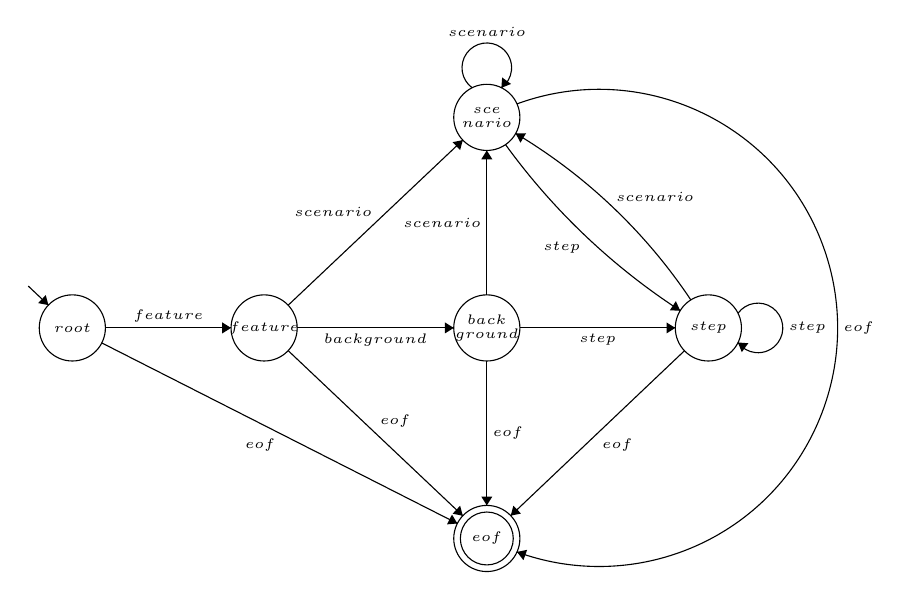
\begin{tikzpicture}[scale=0.14]
	\tiny{
	\tikzstyle{every node}+=[inner sep=0pt]
	\draw [black] (5.2,-29) circle (3);
	\draw (5.2,-29) node {$root$};
	\draw [black] (22.6,-29) circle (3);
	\draw (22.6,-29) node {$feature$};
	\draw [black] (42.8,-29) circle (3);
	\draw (42.8,-29) node {$\substack{back\\ground}$};
	\draw [black] (42.8,-48.1) circle (3);
	\draw (42.8,-48.1) node {$eof$};
	\draw [black] (42.8,-48.1) circle (2.4);
	\draw [black] (42.8,-9.9) circle (3);
	\draw (42.8,-9.9) node {$\substack{sce\\nario}$};
	\draw [black] (62.9,-29) circle (3);
	\draw (62.9,-29) node {$step$};
	\draw [black] (8.2,-29) -- (19.6,-29);
	\fill [black] (19.6,-29) -- (18.8,-28.5) -- (18.8,-29.5);
	\draw (13.9,-28.5) node [above] {$feature$};
	\draw [black] (7.87,-30.36) -- (40.13,-46.74);
	\fill [black] (40.13,-46.74) -- (39.64,-45.93) -- (39.19,-46.82);
	\draw (22.24,-39.06) node [below] {$eof$};
	\draw [black] (24.78,-31.06) -- (40.62,-46.04);
	\fill [black] (40.62,-46.04) -- (40.38,-45.13) -- (39.7,-45.85);
	\draw (34.49,-38.07) node [above] {$eof$};
	\draw [black] (25.6,-29) -- (39.8,-29);
	\fill [black] (39.8,-29) -- (39,-28.5) -- (39,-29.5);
	\draw (32.7,-29.5) node [below] {$background$};
	\draw [black] (24.78,-26.94) -- (40.62,-11.96);
	\fill [black] (40.62,-11.96) -- (39.7,-12.15) -- (40.38,-12.87);
	\draw (28.85,-18.97) node [above] {$scenario$};
	\draw [black] (45.421,-11.359) arc (59.16523:33.75739:49.833);
	\fill [black] (45.42,-11.36) -- (45.85,-12.2) -- (46.36,-11.34);
	\draw (58.05,-17.54) node [above] {$scenario$};
	\draw [black] (65.58,-27.677) arc (144:-144:2.25);
	\draw (70.15,-29) node [right] {$step$};
	\fill [black] (65.58,-30.32) -- (65.93,-31.2) -- (66.52,-30.39);
	\draw [black] (41.477,-7.22) arc (234:-54:2.25);
	\draw (42.8,-2.65) node [above] {$scenario$};
	\fill [black] (44.12,-7.22) -- (45,-6.87) -- (44.19,-6.28);
	\draw [black] (42.8,-26) -- (42.8,-12.9);
	\fill [black] (42.8,-12.9) -- (42.3,-13.7) -- (43.3,-13.7);
	\draw (42.3,-19.45) node [left] {$scenario$};
	\draw [black] (45.8,-29) -- (59.9,-29);
	\fill [black] (59.9,-29) -- (59.1,-28.5) -- (59.1,-29.5);
	\draw (52.85,-29.5) node [below] {$step$};
	\draw [black] (60.344,-27.43) arc (-123.00486:-144.07252:59.783);
	\fill [black] (60.34,-27.43) -- (59.95,-26.57) -- (59.4,-27.41);
	\draw (49.6,-21.11) node [below] {$step$};
	\draw [black] (60.73,-31.07) -- (44.97,-46.03);
	\fill [black] (44.97,-46.03) -- (45.9,-45.84) -- (45.21,-45.12);
	\draw (54.64,-39.03) node [below] {$eof$};
	\draw [black] (45.537,-8.677) arc (110.11043:-110.11043:21.643);
	\fill [black] (45.54,-49.32) -- (46.12,-50.07) -- (46.46,-49.13);
	\draw (75.12,-29) node [right] {$eof$};
	\draw [black] (42.8,-32) -- (42.8,-45.1);
	\fill [black] (42.8,-45.1) -- (43.3,-44.3) -- (42.3,-44.3);
	\draw (43.3,-38.55) node [right] {$eof$};
	\draw [black] (1.2,-25.2) -- (3.03,-26.93);
	\fill [black] (3.03,-26.93) -- (2.79,-26.02) -- (2.1,-26.75);
	}
	\end{tikzpicture}
	\caption{The FSM built by Ragel.}
	\label{figure:automaton}
\end{figure}

Consider now, that every state in the automaton shown in Figure \ref{figure:automaton} has a transition that goes to the final state. Hence, we can reduce the graph removing the \textit{eof} state and converting all the states in finals. The result can be seen in Figure \ref{figure:gherkin_fsm_simple}.

\begin{figure}[h!]
	\centering
	\tiny{
	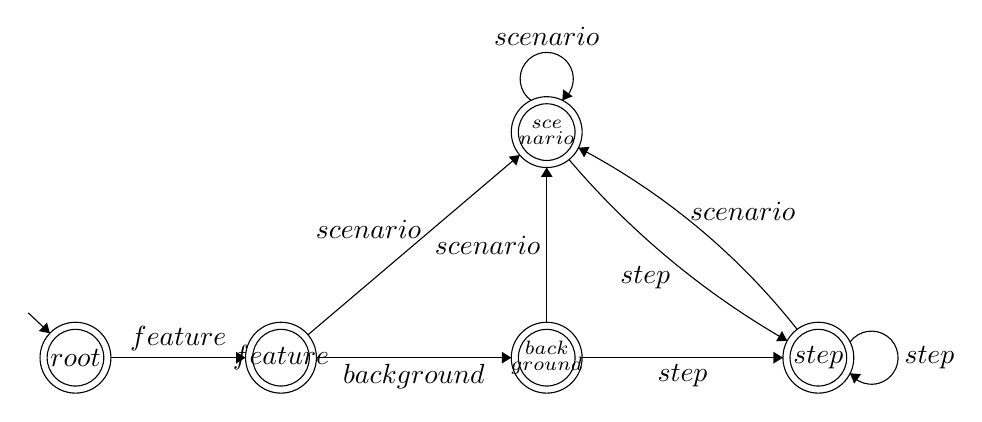
\begin{tikzpicture}[scale=0.15]
	\tikzstyle{every node}+=[inner sep=0pt]
	\draw [black] (5.2,-29) circle (3);
	\draw (5.2,-29) node {$root$};
	\draw [black] (5.2,-29) circle (2.4);
	\draw [black] (22.6,-29) circle (3);
	\draw (22.6,-29) node {$feature$};
	\draw [black] (22.6,-29) circle (2.4);
	\draw [black] (45.1,-29) circle (3);
	\draw (45.1,-29) node {$\substack{back\\ground}$};
	\draw [black] (45.1,-29) circle (2.4);
	\draw [black] (45.1,-9.9) circle (3);
	\draw (45.1,-9.9) node {$\substack{sce\\nario}$};
	\draw [black] (45.1,-9.9) circle (2.4);
	\draw [black] (68.1,-29) circle (3);
	\draw (68.1,-29) node {$step$};
	\draw [black] (68.1,-29) circle (2.4);
	\draw [black] (8.2,-29) -- (19.6,-29);
	\fill [black] (19.6,-29) -- (18.8,-28.5) -- (18.8,-29.5);
	\draw (13.9,-28.5) node [above] {$feature$};
	\draw [black] (25.6,-29) -- (42.1,-29);
	\fill [black] (42.1,-29) -- (41.3,-28.5) -- (41.3,-29.5);
	\draw (33.85,-29.5) node [below] {$background$};
	\draw [black] (24.89,-27.06) -- (42.81,-11.84);
	\fill [black] (42.81,-11.84) -- (41.88,-11.98) -- (42.53,-12.74);
	\draw (30.01,-18.96) node [above] {$scenario$};
	\draw [black] (47.791,-11.224) arc (62.31309:38.27207:57.772);
	\fill [black] (47.79,-11.22) -- (48.27,-12.04) -- (48.73,-11.15);
	\draw (61.7,-17.44) node [above] {$scenario$};
	\draw [black] (70.78,-27.677) arc (144:-144:2.25);
	\draw (75.35,-29) node [right] {$step$};
	\fill [black] (70.78,-30.32) -- (71.13,-31.2) -- (71.72,-30.39);
	\draw [black] (43.777,-7.22) arc (234:-54:2.25);
	\draw (45.1,-2.65) node [above] {$scenario$};
	\fill [black] (46.42,-7.22) -- (47.3,-6.87) -- (46.49,-6.28);
	\draw [black] (45.1,-26) -- (45.1,-12.9);
	\fill [black] (45.1,-12.9) -- (44.6,-13.7) -- (45.6,-13.7);
	\draw (44.6,-19.45) node [left] {$scenario$};
	\draw [black] (48.1,-29) -- (65.1,-29);
	\fill [black] (65.1,-29) -- (64.3,-28.5) -- (64.3,-29.5);
	\draw (56.6,-29.5) node [below] {$step$};
	\draw [black] (65.464,-27.569) arc (-119.74114:-139.6737:69.37);
	\fill [black] (65.46,-27.57) -- (65.02,-26.74) -- (64.52,-27.61);
	\draw (53.44,-21.2) node [below] {$step$};
	\draw [black] (1.2,-25.2) -- (3.03,-26.93);
	\fill [black] (3.03,-26.93) -- (2.79,-26.02) -- (2.1,-26.75);
	\end{tikzpicture}
	}
	\caption{A simplified version of the FSM built by Ragel.}
	\label{figure:gherkin_fsm_simple}
	\vspace{0.2cm}
\end{figure}

While the parsing process is running, the parser sends an event to a Cucumber listener which executes semantic actions for each keyword found.

\newpage
\section{Cucumber}

Cucumber\footnote{\url{https://github.com/cucumber/cucumber}} uses Gherkin to parse feature files in order to execute all the scenarios.

Every time that the Gherkin's parser finds a keyword, it sends to the Cucumber listener that word followed by the plain-text written until the next keyword. This mechanism is made possible because keywords are always followed by plain text (i.e, see Figure \ref{figure:scenario_example_original}). When these values are received by the listener, Cucumber runs a semantic action associated to that keyword. Basically, these actions are functions that build an Abstract Syntax Tree (AST) for each feature file analysed. In particular, every node in the tree has the structure illustrated by Figure \ref{table:node_structure}.

\begin{table}[h!]
	\renewcommand*\arraystretch{1.3}
	\begin{center}
	\begin{tabular}{|c|c|}
		\hline
		\multicolumn{2}{|c|}{\textit{parent}} \\ \hline
		\textit{keyword} & \textit{plaintext} \\ \hline
		\multicolumn{2}{|c|}{$child_1$ ... $child_n$} \\ \hline
	\end{tabular}
	\caption{The structure of nodes in the AST built by Cucumber.}
	\label{table:node_structure}
	\end{center}
\end{table}

The tree is built as following: when the keyword \textit{Feature} is recognized by Gherkin, a new instance of an AST is created and a new node composed by the word Feature and its description is added as root to that tree.
When the word recognized is \textit{Scenario}, a new child node is added to the root node. This node will contain the values Scenario as keyword and the name of the scenario as plain-text. The same process happens when a step keywords is found: all the steps of a scenario becomes children nodes of that scenario node. Steps will be leaf nodes of the tree.

Figure \ref{figure:ast_cucumber} shows the AST built by Cucumber for the feature file shown in Figure \ref{figure:scenario_example_original}.

\begin{figure}[H]
	\centering
	\synttree	[Feature
			    	[Login
				    	[$Step_i$]
				    	[\dots]
				    	[$Step_n$]
					]
			    	[Logout
			    		[$Step_k$]
			    		[\dots]
			       		[$Step_m$]
					]
				]
	\vspace{0.2cm}
	\caption{An example of an Abstract Syntax Tree built by Cucumber.}
	\label{figure:ast_cucumber}
\end{figure}

In the end of the parsing process, Cucumber has an AST instance with the same structure of the feature file parsed.

To execute all the scenarios stored in the AST, Cucumber creates an instance of a \textit{Visitor} class which starts a preorder tree traversal. Each scenario is executed as a separate test case, with no interaction to other scenarios or features. The output produced by Cucumber is the following:

\begin{itemize}
\item If the node visited has the words Feature or Scenarios in the keyword field, the output is the keyword followed by the plain-text as written in the input file.
\item If the node visited has a step keyword in the keyword field, Cucumber tries to match the plain-text with a regular expression written in a step definition file. If a match is found then the test code written into that step definition is executed, otherwise a pending error is raised and the execution is stopped.
\end{itemize}

Cucumber also formats the output on the terminal providing indentation and displaying each step with a color: passing steps are coloured green, failing steps red, and undefined and pending steps yellow. When a step fails or is undefined, Cucumber skips to the next scenario and colors the skipped steps cyan\footnote{\url{https://github.com/cucumber/cucumber/wiki/Step-Definitions}}.

The output of the Cucumber execution of the feature file visible in Figure \ref{figure:scenario_example_original} can be seen in Figure \ref{figure:scenario_example_original_executed}. 

\begin{figure}[h!]
\begin{minted}[fontsize=\small,frame=single]{gherkin}
Feature: Login and logout as collector

  Scenario: Login
    Given I am on the login page
    When I sign in as "collector@example.com"
    Then I should see "Available Offers"

  Scenario: Logout
    Given I am logged in as "collector@example.com"
    When I sign out
    Then I should be redirected to the login page

2 scenarios (2 passed)
6 steps (6 passed)
0m0.010s
\end{minted}
\vspace{-1em}
\caption{The result of the execution of Cucumber.}
\label{figure:scenario_example_original_executed}
\end{figure}

\newpage
\section{SimpleCov}

To gather information about our tests in Bring The Food we use a code coverage analysis tool for Ruby called \textit{SimpleCov}\footnote{\url{https://rubygems.org/gems/simplecov}}. SimpleCov gathers code coverage data from all tests including Cucumber's step definitions, RSpec and Capybara. It analyses which lines of code are covered by tests and then formats the results providing an html output file where the percentage of code coverage can be seen for each Ruby file in the project. We can also see the coverage for categories such as controllers, models, mailers and helpers.

The first time we used SimpleCov in Bring the Food we got the 50\% of code coverage. This result was expected considering the following aspects:

\begin{enumerate}
\item We tested only the main features of the application including the Sign up, the Login, the Logout and other actions such as publishing, booking, editing and deleting food donations.
\item We introduced the BDD technique when most of the application's features were already developed.
\end{enumerate}

If we consider the results provided by this tool, we may infer that the 50\% of our application has been tested.
Unfortunately, in a high-level language like Ruby, some lines of code marked as covered by SimpleCov, may not be tested by test cases. In fact, some of these are marked simply by loading the test environment.

\section{Gems overview}

All the previous gems can be combined in order to enforce the validation of Ruby on Rails web applications.

\begin{table}[h!]
	\vspace{0.2cm}
	\renewcommand*\arraystretch{1.5}
	\begin{center}
	\begin{tabular}{|c|}
		\hline
		SimpleCov \\ \hline
		Gherkin and Cucumber \\ \hline
		RSpec and Capybara \\ \hline
		MiniTest \\ \hline
	\end{tabular}
	\vspace{0.2cm}
	\caption{The BDD gem stack used in Bring The Food.}
	\label{table:structureofgems}
	\end{center}
\end{table}

Table \ref{table:structureofgems} shows how I used those gems: starting from the bottom, where the default MiniTest framework can be seen, going up to the last gem introduced in the Bring The Food development process.


\chapter{The limits of the Cucumber gem}

To reach a satisfactory level of test coverage, and obtain an high percentage value in SimpleCov, testers need to write lots of test cases for each feature. However, managing lots of tests in a single file may be difficult. Consider also that, scenarios may be similar to each other. Hence, the same steps often occur in different scenarios. 

For instance, consider the Login condition: most of our scenarios use it to test features that require a user which is logged in the application. Consequently, also same results can be expected by different test cases (e.g., Login failed with a wrong username, wrong password, wrong username and password). As result, in order to validate little changes, tests repeat other tests or part of them more than once. To better understand this situation, we can define three categories of steps:

\begin{enumerate}
\item \textbf{Category 1}: conditions written to prepare an environment which will be the object of the testing activity. These steps usually start with the word \textit{Given}.
\item \textbf{Category 2}: steps used to test the behavior of features in particular scenarios. These steps are usually written in the middle of test cases and start with the word \textit{When}.
\item \textbf{Category 3}: checks which are used by Cucumber to validate test cases. These steps usually start with the word \textit{Then}.
\end{enumerate}

Every time Cucumber runs a test, steps that belong to both the first and the third category are always defined and executed by many different test cases testing similar functions. Therefore, those steps violate the DRY principle in Ruby, so our goal is to avoid duplicate of them. This provides us with a credible basis to believe that this situation is due to the fact that each scenario is run as a separate test case. 

\section{A real example}

A clear example of the problems mentioned in the previous section is shown in Figure \ref{figure:scenario_example_problems}.

\begin{figure}[H]
\begin{minted}[fontsize=\small,frame=single,linenos=true]{gherkin}
Feature: Example of Collectors' actions

  Scenario: Login
    Given I am on the login page
    When I sign in as "collector@example.com"
    Then I should see "Available Offers"

  Scenario: Logout
    Given I am logged in as "collector@example.com"
    When I sign out
    Then I should be redirected to the login page

  Scenario: Login and Logout
    Given I am on the login page
    When I sign in as "collector@example.com"
    And I sign out
    Then I should be redirected to the login page

  Scenario: A collector creates a donation
    Given I am logged in as "collector@example.com"
    When I publish a new donation
    Then I should see the last donation in the list of donations

  Scenario: A collector creates two donations
    Given I am logged in as "collector@example.com"
    When I publish two new donations
    Then I should see the last 2 donations in the list of donations

  Scenario: A collector creates a donation and then logs out
    Given I am logged in as "collector@example.com"
    When I publish a new donations
    And I sign out
    Then I should be redirected to the login page
\end{minted}
\vspace{-1em}
\caption{Some scenarios repeat steps that has been already executed.}
\label{figure:scenario_example_problems}
\end{figure}

As it can be seen, there are six scenarios that test the following features: login, logout, and the creation of a new donation. In particular, we can note that three of them expect the same page redirect, while four of them have the same initial condition: the login of the user as collector.

Therefore we believe that is crucial to give testers a method which follows the DRY principle allowing an easier and a faster way to write and organize test cases. The solution we found is to extend the Gherkin and Cucumber gems in order to limit step repetitions and to generate test case automatically.

\section{Related work}

Many approaches have been proposed to address the problem of test case generation.

In \cite{automated_test_case_ia}, a method for automatic testing based on an extended IA (EIA) model is provided, while \cite{novel_approach} presents a two-phase approach to generate test cases automatically by analyzing structure of Web applications.

One approach we found similar to our work is \cite{book:towards_paper} because it faces the same problem in terms of Ruby on Rails Web applications. It sketches an algorithm for generating test cases based on uncovered lines of code. To archive this, it automatically writes new step definitions in feature files. In this way, testers write only test code to make pass the steps.

However, our approach is different because the proposed solution allows testers to generate and execute multiple scenarios based on the composition of single test cases.
\chapter{The proposed solution}

\section{Gherkin*}

To allow testers to write test cases that can be automatically executed, it is necessary first to extend Gherkin. We developed \textit{Gherkin*}, which extends the Gherkin language and adds the possibility to link scenarios each others.

Consequently, testers could write some scenarios to test initial conditions and others to test final results. Then, they could write scenarios that test specific behaviour of some features and connect all of them together.

\textit{Gherkin*} adds the new word \textbf{\textit{Next\_Scenario}} to the original set of keywords (see Table \ref{table:gherkin_keywords}). The idea is the following: we want to allow testers to write the keyword \textit{Next\_Scenario} in order to link test cases and avoid step repetitions. This keyword aims to be a link between two test cases and it will be used by \textit{Cucumber*} (see the next section) to execute two or more scenarios in sequence.

If we consider the feature file shown in Figure \ref{figure:scenario_example_original}, the first problem we face is to understand where that keyword may be written respect to the others. In order to solve this issue, we need to define some rules that testers must follow, so we extend the original grammar.

The process of making changes to the Gherkin's language involves little changes to its grammar. However, a grammar extension is not always an easy task: it may contain lots of productions and several terminal symbols. Hence, it can be difficult to find the right place to edit. Moreover, by adding other productions we may generate a completely different language, making the grammar ambiguous or recursive.

To avoid these situations and to validate the new grammar we write tests. There are a lot of scenarios written into the test folder of the Gherkin gem. We use them and we add more tests that check the correctness of the new productions as follows. Given a feature file as input to a scenario, the goal is to check that no parser errors occur for that file.

The first test we write leads us to validate the basics use of our solution. More precisely, we want to test that a \textit{Next\_Scenario} definition may appear after the last step of a \textit{Scenario}. Hence, we write the feature file shown in Figure \ref{figure:scenario_example_next_scenario} and we run the test.

\begin{figure}[H]
\begin{minted}[fontsize=\small,frame=single,linenos=true]{gherkin}
Feature: Login and logout as collector

  Scenario: Login
    Given I am on the login page
    When I sign in as "collector@example.com"
    Then I should see "Available Offers"
  Next_Scenario: Logout

  Scenario: Logout
    Given I am logged in as "collector@example.com"
    When I sign out
    Then I should be redirected to the login page
\end{minted}
\vspace{-1em}
\caption{An example of a feature files.}
\label{figure:scenario_example_next_scenario}
\end{figure}

Obviously, the test fails because the original grammar does not contain productions for the new keyword. To pass the test, we first add some productions to the grammar. Those productions allow the parser to successfully parse new lines that contain the \textit{Next\_Scenario} token followed by a name of one scenario. As we already said, those productions leads also the parser to send an event to the Cucumber*'s listener with both the keyword and the plain-text values parsed in that line.

However, the parser uses also a parsing table to parse feature files, so we need also to extend that table: we add a new row and a new column, both start with the \textit{next\_scenario} word. The highlighted part of the Table \ref{table:parsing_table_gherkin_new_before} shows the first changes applied to the original parsing table. Consider that the position of the new row and the new column is not relevant.

\newcolumntype{a}{>{\columncolor{LightCyan}}l}

\begin{table}[h]
	\renewcommand*\arraystretch{1.5}
	\centering
	\setlength{\arrayrulewidth}{1pt}
	\resizebox{\linewidth}{!}{
	\begin{tabular}{|r|l|l|l|l|a|l|l|l|l|l|l|l|}
	\cline{2-11}
	\multicolumn{1}{r|}{}  	& feature & background & scenario      & scenario\_outline 	& next\_scenario	& examples & step         	& row            	& doc\_string   	& eof \\ \hline
	root             		& feature & E          & E             & E                	& 	           		& E        & E            	& E              	& E            		& eof \\ \hline
	feature          		& E       & background & scenario      & scenario\_outline 	& 	            	& E        & E            	& E              	& E            		& eof \\ \hline
	step             		& E       & E          & scenario      & scenario\_outline 	& 				 	& E        & step         	& step           	& step         		& eof \\ \hline
	outline\_step     		& E       & E          & scenario      & scenario\_outline 	& 				 	& examples & outline\_step 	& outline\_step   	& outline\_step 	& eof \\ \hline
	background       		& E       & E          & scenario      & scenario\_outline 	& 	             	& E        & step         	& E              	& E            		& eof \\ \hline
	scenario         		& E       & E          & scenario      & scenario\_outline 	& 					& E        & step         	& E              	& E            		& eof \\ \hline
	scenario\_outline 		& E       & E          & E             & E                	& 				 	& E        & outline\_step 	& E              	& E            		& eof \\ \hline \rowcolor{LightCyan}
	next\_scenario    		&         &            & 		       & 				 	& 				 	&          &          		&               	&             		&     \\ \hline
	examples        		& E       & E          & E             & E                	& 	            	& E        & E            	& examples\_table 	& E            		& eof \\ \hline
	examples\_table   		& E       & E          & scenario      & scenario\_outline 	& 	             	& examples & E            	& examples\_table 	& E            		& eof \\ \hline
	eof              		& E       & E          & E             & E                	& 	             	& E        & E            	& E              	& E            		& E   \\ \hline
	\end{tabular}
	}
	\caption{The first changes applied to the original parsing table of Gherkin*.}
	\label{table:parsing_table_gherkin_new_before}
\end{table}

\noindent Once the parsing table contains the definition of the \textit{Next\_Scenario} keyword, it is necessary to understand which values should be written into the highlighted cells. As we already explained in Section 2.4, each cell define a rule that must be obeyed by testers. More precisely, each cell represent a transition in the FSM produced by Ragel.

If we consider the feature file shown in Figure \ref{figure:scenario_example_next_scenario}, the new parsing table should have a rule that allow testers to write the new keyword after the last step of the first scenario. We add the keyword \textit{next\_scenario} in the cell corresponds to the row \textit{step} and the column \textit{next\_scenario}. Furthermore, we do not want that the opposite way happens, allowing therefore \textit{step} definitions after a \textit{Next\_Scenario} line. This situation can be avoided by adding an Expected Error (E) value in the cell which cross the row \textit{next\_scenario} and the column \textit{step}. Moreover, to allow that a \textit{Next\_Scenario} definition can be followed by a \textit{Scenario}, it is necessary to add one more rule in the parsing table. So, we add the keyword \textit{next\_scenario} in the cell corresponds to the row \textit{next\_scenario} and the column \textit{scenario}. The results can be seen in Table \ref{table:parsing_table_gherkin_new_first_step}.

\begin{table}[h]
	\renewcommand*\arraystretch{1.5}
	\centering
	\resizebox{\linewidth}{!}{
	\begin{tabular}{|r|l|l|l|l|l|l|l|l|l|l|l|l|}
	\cline{2-11}
	\multicolumn{1}{r|}{}	& feature & background & scenario      & scenario\_outline 	& next\_scenario	& examples & step         	& row            	& doc\_string   	& eof \\ \hline
	root             		& feature & E          & E             & E                	& 	           		& E        & E            	& E              	& E            		& eof \\ \hline
	feature          		& E       & background & scenario      & scenario\_outline 	& 	            	& E        & E            	& E              	& E            		& eof \\ \hline
	step             		& E       & E          & scenario      & scenario\_outline 	& \cellcolor{kellygreen}next\_scenario	& E        & step         	& step           	& step         		& eof \\ \hline
	outline\_step     		& E       & E          & scenario      & scenario\_outline 	& 				 	& examples & outline\_step 	& outline\_step   	& outline\_step 	& eof \\ \hline
	background       		& E       & E          & scenario      & scenario\_outline 	& 	             	& E        & step         	& E              	& E            		& eof \\ \hline
	scenario         		& E       & E          & scenario      & scenario\_outline 	& 					& E        & step         	& E              	& E            		& eof \\ \hline
	scenario\_outline 		& E       & E          & E             & E                	& 				 	& E        & outline\_step 	& E              	& E            		& eof \\ \hline
	next\_scenario    		&         &            & \cellcolor{kellygreen}scenario &  	& 				 	&          & \cellcolor{ruddy}E         		&               	&             		&     \\ \hline
	examples        		& E       & E          & E             & E                	& 	            	& E        & E            	& examples\_table 	& E            		& eof \\ \hline
	examples\_table   		& E       & E          & scenario      & scenario\_outline 	& 	             	& examples & E            	& examples\_table 	& E            		& eof \\ \hline
	eof              		& E       & E          & E             & E                	& 	             	& E        & E            	& E              	& E            		& E   \\ \hline
	\end{tabular}
	}
	\caption{The details of a rule in the parsing table of Gherkin*.}
	\label{table:parsing_table_gherkin_new_first_step}
\end{table}

These three rules are necessary to allow testers to write a feature file like the one shown in Figure \ref{figure:scenario_example_next_scenario}. However, to check if the parser can parse that file, we run another time all the tests, and this time they pass. Afterwards we introduce other rules that allow feature files to have multiple \textit{Next\_Scenario} definitions within the same Scenario. An example use is login scenarios which are used not only to check if the login feature works as expected but also as conditions for some other scenarios or features. We also allow testers to write the new keyword in \textit{Scenario Outline} contexts. The reason, as we already said, is that \textit{Scenario} and \textit{Scenario Outline} are test case so in the final parsing table shown in Figure \ref{table:parsing_table_gherkin_new_after} we can see that there is a rule for both. The \textit{eof} value in the last column allow the word \textit{Next\_Scenario} to be the last keyword in a feature file. In all the remaining cells we set the value \textit{E}.

\newcolumntype{a}{>{\columncolor{LightCyan}}l}

\begin{table}[H]
	\renewcommand*\arraystretch{1.5}
	\centering
	\resizebox{\linewidth}{!}{
	\begin{tabular}{|r|l|l|l|l|l|l|l|l|l|l|l|l|}
	\cline{2-11}
	\multicolumn{1}{r|}{}	& feature 	& background 	& scenario      					& scenario\_outline 						& next\_scenario						& examples & step         	& row            	& doc\_string   	& eof \\ \hline
	root             		& feature 	& E          	& E             					& E                							& E            							& E        & E            	& E              	& E            		& eof \\ \hline
	feature          		& E       	& background 	& scenario      					& scenario\_outline 						& E             						& E        & E            	& E              	& E            		& eof \\ \hline
	step             		& E       	& E          	& scenario      					& scenario\_outline 						& \cellcolor{kellygreen}next\_scenario 	& E        & step         	& step           	& step         		& eof \\ \hline
	outline\_step     		& E      	& E          	& scenario      					& scenario\_outline 						& \cellcolor{kellygreen}next\_scenario 	& examples & outline\_step 	& outline\_step   	& outline\_step 	& eof \\ \hline
	background       		& E       	& E          	& scenario      					& scenario\_outline 						& E             						& E        & step         	& E              	& E            		& eof \\ \hline
	scenario         		& E     	& E          	& scenario     						& scenario\_outline 						& \cellcolor{kellygreen}next\_scenario	& E        & step         	& E              	& E            		& eof \\ \hline
	scenario\_outline 		& E     	& E          	& E             					& E                							& \cellcolor{kellygreen}next\_scenario 	& E        & outline\_step 	& E              	& E            		& eof \\ \hline
	next\_scenario    		& E 		& E 			& \cellcolor{kellygreen}scenario 	& \cellcolor{kellygreen}scenario\_outline 	& \cellcolor{kellygreen}next\_scenario 	& E        & E         		& E              	& E            		& \cellcolor{kellygreen}eof \\ \hline
	examples        		& E 		& E          	& E             					& E                							& E             						& E        & E            	& examples\_table 	& E            		& eof \\ \hline
	examples\_table   		& E    		& E          	& scenario      					& scenario\_outline 						& E             						& examples & E            	& examples\_table 	& E            		& eof \\ \hline
	eof              		& E     	& E          	& E             					& E                							& E             						& E        & E            	& E              	& E            		& E   \\ \hline
	\end{tabular}
	}
	\caption{The parsing table used by Gherkin*.}
	\label{table:parsing_table_gherkin_new_after}
\end{table}

\noindent Consequently, also the FSM produced by Ragel must respect all those new rules. 

\begin{figure}[h!]
	\centering
	\tiny{
	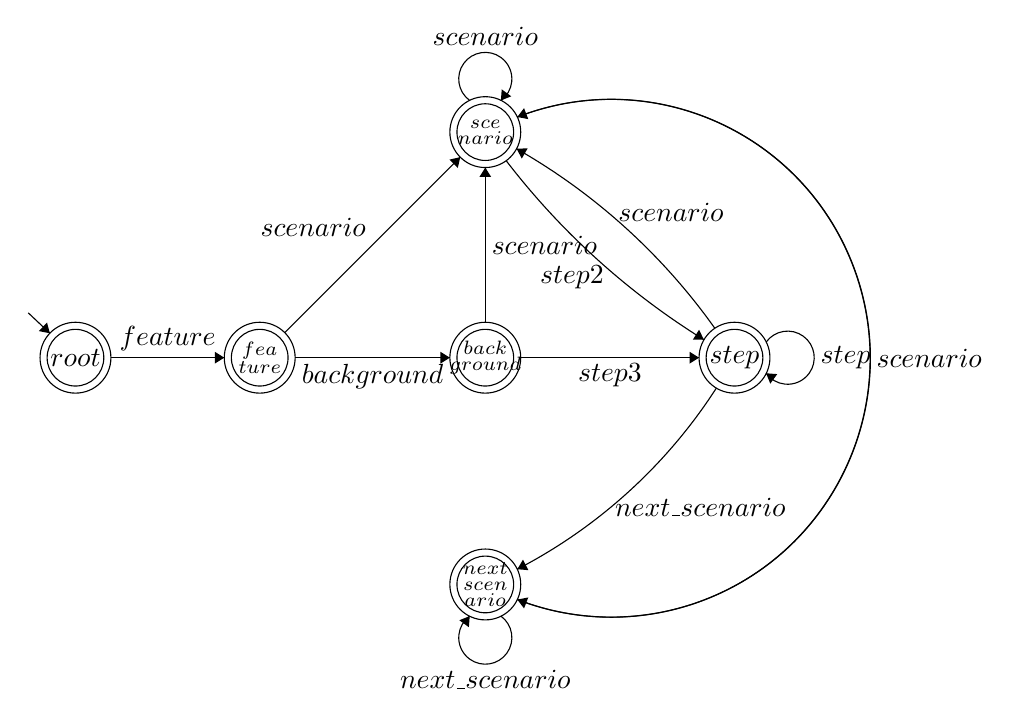
\begin{tikzpicture}[scale=0.15]
	\tikzstyle{every node}+=[inner sep=0pt]
	\draw [black] (5.4,-29) circle (3);
	\draw (5.4,-29) node {$root$};
	\draw [black] (5.4,-29) circle (2.4);
	\draw [black] (21,-29) circle (3);
	\draw (21,-29) node {$\substack{fea\\ture}$};
	\draw [black] (21,-29) circle (2.4);
	\draw [black] (40.1,-29) circle (3);
	\draw (40.1,-29) node {$\substack{back\\ground}$};
	\draw [black] (40.1,-29) circle (2.4);
	\draw [black] (40.1,-9.9) circle (3);
	\draw (40.1,-9.9) node {$\substack{sce\\nario}$};
	\draw [black] (40.1,-9.9) circle (2.4);
	\draw [black] (61.2,-29) circle (3);
	\draw (61.2,-29) node {$step$};
	\draw [black] (61.2,-29) circle (2.4);
	\draw [black] (40.1,-48.2) circle (3);
	\draw (40.1,-48.2) node {$\substack{next\\scen\\ario}$};
	\draw [black] (40.1,-48.2) circle (2.4);
	\draw [black] (8.4,-29) -- (18,-29);
	\fill [black] (18,-29) -- (17.2,-28.5) -- (17.2,-29.5);
	\draw (13.2,-28.5) node [above] {$feature$};
	\draw [black] (24,-29) -- (37.1,-29);
	\fill [black] (37.1,-29) -- (36.3,-28.5) -- (36.3,-29.5);
	\draw (30.55,-29.5) node [below] {$background$};
	\draw [black] (23.12,-26.88) -- (37.98,-12.02);
	\fill [black] (37.98,-12.02) -- (37.06,-12.23) -- (37.77,-12.94);
	\draw (30.03,-17.97) node [left] {$scenario$};
	\draw [black] (42.747,-11.31) arc (60.31359:35.38279:52.45);
	\fill [black] (42.75,-11.31) -- (43.19,-12.14) -- (43.69,-11.27);
	\draw (55.82,-17.5) node [above] {$scenario$};
	\draw [black] (63.88,-27.677) arc (144:-144:2.25);
	\draw (68.45,-29) node [right] {$step$};
	\fill [black] (63.88,-30.32) -- (64.23,-31.2) -- (64.82,-30.39);
	\draw [black] (38.777,-7.22) arc (234:-54:2.25);
	\draw (40.1,-2.65) node [above] {$scenario$};
	\fill [black] (41.42,-7.22) -- (42.3,-6.87) -- (41.49,-6.28);
	\draw [black] (40.1,-26) -- (40.1,-12.9);
	\fill [black] (40.1,-12.9) -- (39.6,-13.7) -- (40.6,-13.7);
	\draw (40.6,-19.45) node [right] {$scenario$};
	\draw [black] (43.1,-29) -- (58.2,-29);
	\fill [black] (58.2,-29) -- (57.4,-28.5) -- (57.4,-29.5);
	\draw (50.65,-29.5) node [below] {$step3$};
	\draw [black] (58.614,-27.48) arc (-121.81606:-142.48757:62.943);
	\fill [black] (58.61,-27.48) -- (58.2,-26.63) -- (57.67,-27.48);
	\draw (47.43,-21.15) node [below] {$step2$};
	\draw [black] (1.4,-25.2) -- (3.23,-26.93);
	\fill [black] (3.23,-26.93) -- (2.99,-26.02) -- (2.3,-26.75);
	\draw [black] (41.423,-50.88) arc (54:-234:2.25);
	\draw (40.1,-55.45) node [below] {$next\_scenario$};
	\fill [black] (38.78,-50.88) -- (37.9,-51.23) -- (38.71,-51.82);
	\draw [black] (59.662,-31.575) arc (-32.78023:-62.61835:44.255);
	\fill [black] (42.81,-46.91) -- (43.75,-46.99) -- (43.29,-46.1);
	\draw (58.31,-40.83) node [below] {$next\_scenario$};
	\draw [black] (42.813,-8.625) arc (111.25837:-111.25837:21.917);
	\fill [black] (42.81,-49.48) -- (43.38,-50.23) -- (43.74,-49.3);
	\draw (73.18,-29.05) node [right] {$scenario$};
	\draw [black] (42.812,-8.623) arc (111.30366:-111.30366:21.926);
	\fill [black] (42.81,-8.62) -- (43.74,-8.8) -- (43.38,-7.87);
	\end{tikzpicture}
	}
	\vspace{0.1cm}
	\caption{The FSM built by Ragel has now a new state and new transitions.}
	\label{figure:gherkin_automaton_simple_with_next_scenario}
	\vspace{0.2cm}
\end{figure}

\noindent In this way Gherkin* gives Cucumber* a new way to generate scenarios that are not directly written by testers.

\newpage
\section{Cucumber*}

Thanks to Gherkin*, we are now able to parse feature files which contain also the new keyword. The next problem we face is how we can extend Cucumber in order to archive the following goals:

\begin{enumerate}
\item \textbf{To execute scenarios written in feature files}. The results of the execution of those scenarios must be the same both using Cucumber* and the original gem.
\item \textbf{To generate scenarios which are not written in feature files}. Cucumber* should be able to automatically generate new scenarios and execute them in the same way as the written scenarios.
\end{enumerate}

\noindent The flow that Cucumber* follows in order to generate new scenarios can be divided into three main steps:

\begin{enumerate}
\item \textbf{Graph generation}: Cucumber* creates a graph where each node is a test case. Edges between two test cases exist only if a \textit{Next\_Scenario} definition is written in the first node and contains the name of the second one.
\item \textbf{Test case paths detection}: every reachable node in the graph is traversed in order to obtain a set of test case paths.
\item \textbf{Scenario generation}: A new scenario is generated for each path in the graph.
\end{enumerate}

\noindent The focus of the next sections is to explain the techniques used by Cucumber* to generate and execute test case paths.

\newpage
\subsection{Graph generation}

To generate new test cases, we developed Cucumber*, which builds a graph for each feature file where every scenario is a node and every \textit{Next\_Scenario} definition is an edge.

The productions of the grammar allow the parser to recognize lines that contain keywords of the language and at the same time to run semantic actions for those words. More precisely, when the parser is parsing the keyword \textit{Scenario}, Cucumber* uses the existing semantic action for that keyword to add a node to the graph. 

Since the number of scenarios in a feature file may be high, we need to choose how scenarios can be represent as nodes in a graph. The first natural choice is to use a progressive number strategy that associates each scenario to a number. However, in this way some information about scenarios is lost and we have no way to recognize a scenario from a number. To solve this problem we label nodes with the names of the scenarios. In this way, if testers use a short and unique name for each scenario in a feature file, we can searching for a scenario in the graph by looking for its name.

To generate edges we write a semantic action for the new keyword. In this way, when the word \textit{Next\_Scenario} is recognized, we are able to define the starting and the ending nodes of edges as following: while the starting one is the last node added, the ending one is a node labelled by the plain-text that follows the word \textit{Next\_Scenario}.

A problem we face is that the ending node may not exist yet in the graph. For instance consider Figure \ref{figure:scenario_example_next_scenario}: when the \textit{Next\_Scenario} word is parsed, the graph contains only the node labelled by ``Login''. We solve this problem considering that now we are able to recognize if a scenario is already stored in the graph by looking for a node labelled by its name. Hence, two situation must be considered:

\begin{enumerate}
\item The graph contains the destination node, so Cucumber* simply adds an edge between those two nodes.
\item The graph does not contain the destination node, so Cucumber* creates a new one. Note that Cucumber* knows how to label that node because the parser sent an event to the Cucumber*'s listener with both keyword and plain-text values. After that, Cucumber* adds and edge between the parent node and the last created one.
\end{enumerate}

The solution we designed to solve this problem leads us to create an oriented graph by assuming that all the scenarios which are the destination of \textit{Next\_Scenario} definitions must be defined in the same file. This is a little limitation of our prototype. However, we are planning to extend this vision by allowing testers to define links between scenarios written in different feature files.

\noindent The algorithm for building the graph starting from a feature file is shown below.

\vspace{0.2cm}
\begin{algorithm}[H]
	\KwIn{A feature file $F$}
	\KwOut{A graph $G$}
	Let $G \leftarrow \emptyset$\;
	Let $S$ be the set of all scenarios in $F$\;
	\ForEach{$scenario$ in $S$}{
		$G$.add\_node($scenario$)\;
		Let $D$ be the set of all the $Next\_Scenario$ definitions in $scenario$\;
		\ForEach{$d$ in $D$}{
			Let $next\_scenario$ be the name of the scenario which appears after the Next\_Scenario keyword\;
			\If{$next\_scenario$ is not already in $G$ }{
				$G$.add\_node($next\_scenario$)\;
	 		}
	 		$G$.add\_edge($scenario$, $next\_scenario$)\;
		}
	}
	\textbf{return} $G$\;
	\vspace{0.2cm}
	\caption{Algorithm for building the graph of test cases.}
\end{algorithm}
\vspace{0.2cm}

Note that, if the feature file given in input to the algorithm does not contain \textit{Next\_Scenario} definitions, the corresponding graph will not have edges, and no one test case path will be found during the test case paths detection phase. In other words, if the file is written in the Gherkin language, Cucumber* will produce the same output of Cucumber. Figure \ref{figure:cucumber_flow} shows an example of how Cucumber* builds a graph starting from a feature file.

\begin{figure}[H]
\centering
\begin{subfigure}[b]{0.49\textwidth}
\begin{minted}[fontsize=\small]{gherkin}
Feature: Example of Feature

  Scenario: s1
    Next_Scenario: s2
    Next_Scenario: s3
    Next_Scenario: s4

  Scenario: s2
    Next_Scenario: s4

  Scenario: s3
    Next_Scenario: s4

  Scenario: s4
\end{minted}
	\caption{An extended Feature file.}
	\label{figure:feature_file_example}
\end{subfigure}
\begin{subfigure}[b]{0.49\textwidth}
	\centering
	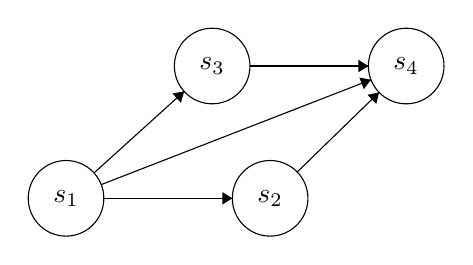
\begin{tikzpicture}[scale=0.16]
	\tikzstyle{every node}+=[inner sep=0pt]
	\draw [black] (3.4,-18) circle (3);
	\draw (3.4,-18) node {$s_1$};
	\draw [black] (19.6,-18) circle (3);
	\draw (19.6,-18) node {$s_2$};
	\draw [black] (30.4,-7.5) circle (3);
	\draw (30.4,-7.5) node {$s_4$};
	\draw [black] (15,-7.5) circle (3);
	\draw (15,-7.5) node {$s_3$};
	\draw [black] (6.4,-18) -- (16.6,-18);
	\fill [black] (16.6,-18) -- (15.8,-17.5) -- (15.8,-18.5);
	\draw [black] (21.75,-15.91) -- (28.25,-9.59);
	\fill [black] (28.25,-9.59) -- (27.33,-9.79) -- (28.02,-10.51);
	\draw [black] (5.62,-15.99) -- (12.78,-9.51);
	\fill [black] (12.78,-9.51) -- (11.85,-9.68) -- (12.52,-10.42);
	\draw [black] (18,-7.5) -- (27.4,-7.5);
	\fill [black] (27.4,-7.5) -- (26.6,-7) -- (26.6,-8);
	\draw [black] (6.2,-16.91) -- (27.6,-8.59);
	\fill [black] (27.6,-8.59) -- (26.68,-8.41) -- (27.04,-9.34);
	\end{tikzpicture}
	\vspace{0.4cm}
	\caption{The corresponding graph.}
	\label{figure:graph_example}
\end{subfigure}
\caption{An example of graph generated by Cucumber*.}
\label{figure:cucumber_flow}
\end{figure}

\subsection{Test case paths detection}

Once the parsing process of a feature file ends, the final graph is made up by nodes (scenarios) and edges (links between two scenarios). To understand how many scenarios can be generated, we need to know how many test paths there are in the graph. A test case path in a graph is a sequence of test cases (scenarios) that are executed visiting one path. Figure \ref{figure:test_case_path_example} shows an example of a test case path.

\begin{figure}[H]
	\centering
	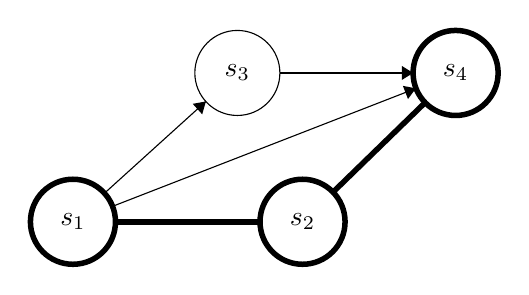
\begin{tikzpicture}[scale=0.18]
	\tikzstyle{every node}+=[inner sep=0pt]
	\draw [black, line width=0.7mm] (3.4,-18) circle (3);
	\draw (3.4,-18) node {$s_1$};
	\draw [black, line width=0.7mm] (19.6,-18) circle (3);
	\draw (19.6,-18) node {$s_2$};
	\draw [black, line width=0.7mm] (30.4,-7.5) circle (3);
	\draw (30.4,-7.5) node {$s_4$};
	\draw [black] (15,-7.5) circle (3);
	\draw (15,-7.5) node {$s_3$};
	\draw [black, line width=0.7mm] (6.4,-18) -- (16.6,-18);
	\draw [black, line width=0.7mm] (21.75,-15.91) -- (28.25,-9.59);
	\draw [black] (5.62,-15.99) -- (12.78,-9.51);
	\fill [black] (12.78,-9.51) -- (11.85,-9.68) -- (12.52,-10.42);
	\draw [black] (18,-7.5) -- (27.4,-7.5);
	\fill [black] (27.4,-7.5) -- (26.6,-7) -- (26.6,-8);
	\draw [black] (6.2,-16.91) -- (27.6,-8.59);
	\fill [black] (27.6,-8.59) -- (26.68,-8.41) -- (27.04,-9.34);
	\end{tikzpicture}
	\vspace{0.3cm}
	\caption{An example of a test case path.}
	\label{figure:test_case_path_example}
\end{figure}

The problem of finding test cases paths starting from a graph is known as a graph coverage problem. It can be solved by choosing the best \textit{test coverage criterion} that fits our needs. There are a several of criteria we can consider for our work: Node Coverage (NC), Edge Coverage (EC), Edge-Pair Coverage (EPC), Simple Round Trip Coverage (SRTC), Complete Round Trip Coverage (CRTC), Prime Path Coverage (PPC) \cite[p. 25-42]{book:introduction_to_software_testing}. These criteria can be implemented extending common algorithm such as the Breadth-first search (BFS) or the Depth-first search (DFS). Furthermore, each criterion defines test requirements (TR) in terms of properties of test paths in a graph. For instance, a typical one is met by visiting a particular node or edge.

Our TR is to cover all the possible test paths in the graph generated in the previous step. The only criterion that meets our requirement is the Complete Path Coverage (CPC). However, this method is not feasible for graphs with cycles\cite[p. 36]{book:introduction_to_software_testing}. In fact, graph with loops has an infinite number of paths, so our TR can not be satisfied.

In order to archive the goal of obtaining test case paths from the graph we use a Breadth-first search visit, assuming that the graph in input has no cycles. This is another limit we post to our prototype. However, it is necessary to solve the problem of the infeasible paths in the early phase of the development. Moreover, we plan to use the Prime Path Coverage (PPC, \cite[p. 36]{book:introduction_to_software_testing}) criterion in the near future for finding prime test paths. According to \cite{book:introduction_to_software_testing}, the advantages are:

\begin{enumerate}
\item The process is guaranteed to terminate because the length of the longest possible prime path is the number of nodes.
\item It can be computed by a simple dynamic programming algorithm.
\item The algorithm requires loops to be executed.
\end{enumerate}

The Breath-First search algorithm we implemented is shown below. We assume that there is a \textit{.last\_path()} method which gets the last subset added in the $curr$ set, and a \textit{.last\_node()} method which obtains the last node added in a set of sub paths.

\vspace{0.4cm}
\begin{algorithm}[H]
	\KwIn{A graph $G$}
	\KwIn{An initial node $n$}
	\KwOut{A list of paths $P$}
	Mark $n$ as visited\;
	Let $Q$ a queue\;
	Let $P$ be the set of final test case paths in $G$\;
	$Q$.push([$n$])\;
	$P \leftarrow \emptyset$\;

	\While{$Q$ is not empty}{
		Let $curr \leftarrow Q$.pop()\;
		Mark last node of $curr$.last\_path() as visited\;
		\If{$curr$.last\_path().adj() is empty}{
			$P$.add\_subset($curr$)\;
		}
		\ForEach {$v \in curr$.last\_path().adj()}{
			Let $tmp\_path \leftarrow curr$\;
			$tmp\_path$.insert($v$)\;
			\uIf{$v$ is not visited}{
				$Q$.push($tmp\_path$)\;
			}
			\Else{
				$P$.add\_subset($tmp\_path$)\;
			}
		}
	}
	\textbf{return} $P$\;
	\vspace{0.2cm}
	\caption{Algorithm for obtaining a list of test paths from a graph.}
\end{algorithm}
\vspace{0.4cm}

Assuming the graph in Figure \ref{figure:graph_example} and the initial node $s_1$ as inputs to the algorithm above, the result set of test case paths is the following:
\begin{center}
$P = \Set{ \Set{s_1,s_3,s_4}, \Set{s_1,s_4}, \Set{s_1,s_2,s_4} }$ \nonumber
\end{center}

\newpage
\subsection{Scenario generation}

To generate new test cases we use the set of unique paths $P$ as input. More precisely, each path will be considered as a new scenario that will be executed by Cucumber*. The crucial part of this process is to understand how new scenarios can be created for each path in $P$.

To understand how we can define a scenario that is made up by other scenarios, we consider every test case as a set of steps. For instance if we consider the scenarios in the subset $\Set{s_1,s_4}$, we can define the following sets of steps:
\begin{align}
s_1 &= \Set{Step_i, \dots, Step_n} \nonumber \\
s_4 &= \Set{Step_k, \dots, Step_m} \nonumber
\end{align}
The idea is to create a new scenario which is composed by the union of all the steps included in $s_1$ and $s_4$. As result, we obtain one single set, maintaining the order between subsets.
\begin{align}
Scenario =& \Set{Step_i, \dots, Step_n} \cup \Set{Step_k, \dots, Step_m} \nonumber \\
=& \Set{Step_i, \dots, Step_n, Step_k, \dots, Step_m} \nonumber
\end{align}
Now that we know how to compose scenarios in a single one, we have to understand how the scenario defined above can be executed by Cucumber*. The solution to this problem can be found considering the AST explained in Section 2.5. To allow Cucumber* to execute new scenarios, we need to add them as children of the root node \textit{Feature}. Moreover, the new nodes must keep the structure defined by the Table \ref{table:node_structure}. Hence, we need a keyword and a plain-text description for each composition.

The keyword problem is solved because we are adding new scenarios to the tree, so we can simply set their keywords to \textit{Scenario}. On the other side, their plain-text values are more difficult to find because each path crossed by the algorithm should have a meaningful name. The reason is that, testers should be able to recognize instantaneously which test case path is failed. A solution we found is to concatenate the names of the single scenarios cross the path using the symbol ``$\rightarrow$'' as follows:
\begin{center}
$scenario_1 \rightarrow scenario_2 \rightarrow \dots \rightarrow scenarios_n$ \nonumber
\end{center}
In our case the plain-text values will result the following:
\begin{center}
$Names = \Set{ \Set{s_1 \rightarrow s_3 \rightarrow s_4}, \Set{s_1 \rightarrow s_4}, \Set{s_1 \rightarrow s_2 \rightarrow s_4} }$
\end{center}

Once Cucumber* has the names of the new scenarios, a new node for each one is added to the AST. However, the nodes have no children, so no steps are executed for those scenarios. To add all the steps as children of the new scenarios, it is necessary to find each step node in the AST. The tree is visited and all the nodes found are cloned and added as children of the right scenario. The result of the final AST can be visible in Figure \ref{figure:ast_cucumber_with_link}.

\begin{figure}[h!]
	\centering
	\vspace{0.1cm}
	\synttree[Feature
					[Login]
					[Logout]
					[Login$\rightarrow$Logout
					[$Step_i$]
						[\dots]
						[$Step_n$]
						[$Step_k$]
						[\dots]
						[$Step_m$]
					]
				]
	\vspace{0.2cm}
	\caption{An example of an Abstract Syntax Tree built by Cucumber*.}
	\label{figure:ast_cucumber_with_link}
\end{figure}

The algorithm which adds new scenarios to the AST is written above. The input are the set of paths produced by the previous step and the AST resulted from the parsing of a feature file.

\vspace{0.4cm}
\begin{algorithm}[H]
	\KwIn{A set of paths $P$, An AST $T$}
	\KwOut{An AST $T$ which contains also generated scenarios}
	Let $r$ be the root of $T$\;
	\ForEach {$p \in P$}{
		Let $name$ be the name of the path\;
		$T$.add\_node\_to\_root(``Scenario'', $name$)\;
		\ForEach {$node \in p$}{
			Let $S$ be the set of steps in $node$\;
			\ForEach {$step \in S$}{
				$step\_node \leftarrow T$.find\_node($step$)\;
				$t$.add\_child($step\_node$)\;
			}
		}
	}
	\textbf{return} $T$\;
	\vspace{0.2cm}
	\caption{Algorithm for generating new scenarios.}
\end{algorithm}
\vspace{0.4cm}

Finally, when the AST is complete and every test case path is added to the tree, Cucumber* executes all the scenarios in the tree by visiting it. No other operations are needed and Cucumber* shows on the output all the scenarios that belong to the tree. An example output of Cucumber* can be seen in Figure \ref{figure:scenario_example_next_scenario_executed}.

As can be seen, no \textit{Next\_Scenario} definitions appear in the output. The number of executed scenarios is equal to:
\begin{center}
Number of written scenarios + $|P|$
\end{center}

\newpage
\begin{figure}[H]
\begin{minted}[fontsize=\small,frame=single]{gherkin}
Feature: Login and logout as collector

  Scenario: Login
    Given I am on the login page
    When I sign in as "collector@example.com"
    Then I should see "Available Offers"

  Scenario: Logout
    Given I am logged in as "collector@example.com"
    When I sign out
    Then I should be redirected to the login page

  Scenario: Login->Logout
    Given I am on the login page
    When I sign in as "collector@example.com"
    Then I should see "Available Offers"
    Given I am logged in as "collector@example.com"
    When I sign out
    Then I should be redirected to the login page

3 scenarios (3 passed)
12 steps (12 passed)
0m0.011s
\end{minted}
\vspace{-1em}
\caption{The result of the execution of Cucumber*.}
\label{figure:scenario_example_next_scenario_executed}
\end{figure}

\newpage
\section{Results}

Figure \ref{figure:kaboom} shows how the feature file shown in Figure \ref{figure:scenario_example_problems} can be rewritten using Gherkin* and Cucumber*.

\begin{figure}[H]
\begin{minted}[fontsize=\small,frame=single,linenos=true]{gherkin}
Feature: Example of Collectors’ actions

  Scenario: Login
    Given I am on the login page
    When I sign in as "collector@example.com"
    Then I should see "Available Offers"
  Next_Scenario: One donation
  Next_Scenario: Two donations
  Next_Scenario: Logout

  Scenario: One donation
    When I publish a new donation
    Then I should see the last donation in the list of donations
  Next_Scenario: Two donations
  Next_Scenario: Logout

  Scenario: Two donations
    When I publish two new donations
    Then I should see the last 2 donations in the list of donations
  Next_Scenario: Logout

  Scenario: Logout
    When I sign out
  Next_Scenario: Redirect

  Scenario: Redirect
    Then I should be redirected to the login page
\end{minted}
\vspace{-1em}
\caption{How a feature file can be written using Gherkin*.}
\label{figure:kaboom}
\end{figure}

We note that two scenarios have been removed because we can execute the same actions by compose scenarios that are written in this file. Moreover, to avoid step duplication, we wrote a new scenario to test the redirect to the login page. All the written scenarios focus on steps that belong to the second category. As result, no duplicate steps occur.

In this feature file there are five \textit{Scenario} and seven \textit{Next\_Scenario} definitions. Hence, the result graph shown in Figure \ref{figure:final_example} has five nodes and seven edges.

\begin{figure}[H]
	\centering
	\tiny{
	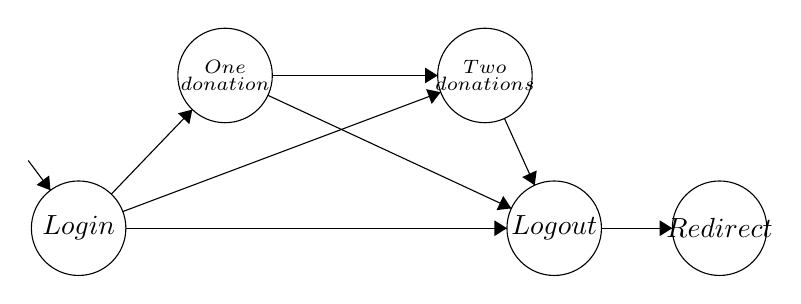
\begin{tikzpicture}[scale=0.2]
	\tikzstyle{every node}+=[inner sep=0pt]
	\draw [black] (13.9,-3.8) circle (3);
	\draw (13.9,-3.8) node {$\substack{One\\donation}$};
	\draw [black] (4.6,-13.5) circle (3);
	\draw (4.6,-13.5) node {$Login$};
	\draw [black] (30.4,-3.8) circle (3);
	\draw (30.4,-3.8) node {$\substack{Two\\donations}$};
	\draw [black] (34.8,-13.5) circle (3);
	\draw (34.8,-13.5) node {$Logout$};
	\draw [black] (45.3,-13.5) circle (3);
	\draw (45.3,-13.5) node {$Redirect$};
	\draw [black] (6.68,-11.33) -- (11.82,-5.97);
	\fill [black] (11.82,-5.97) -- (10.91,-6.2) -- (11.63,-6.89);
	\draw [black] (16.9,-3.8) -- (27.4,-3.8);
	\fill [black] (27.4,-3.8) -- (26.6,-3.3) -- (26.6,-4.3);
	\draw [black] (31.64,-6.53) -- (33.56,-10.77);
	\fill [black] (33.56,-10.77) -- (33.69,-9.83) -- (32.77,-10.25);
	\draw [black] (37.8,-13.5) -- (42.3,-13.5);
	\fill [black] (42.3,-13.5) -- (41.5,-13) -- (41.5,-14);
	\draw [black] (7.41,-12.44) -- (27.59,-4.86);
	\fill [black] (27.59,-4.86) -- (26.67,-4.67) -- (27.02,-5.61);
	\draw [black] (7.6,-13.5) -- (31.8,-13.5);
	\fill [black] (31.8,-13.5) -- (31,-13) -- (31,-14);
	\draw [black] (1.4,-9.2) -- (2.81,-11.09);
	\fill [black] (2.81,-11.09) -- (2.73,-10.15) -- (1.93,-10.75);
	\draw [black] (16.62,-5.06) -- (32.08,-12.24);
	\fill [black] (32.08,-12.24) -- (31.56,-11.45) -- (31.14,-12.35);
	\end{tikzpicture}
	}
	\caption{The graph built by Cucumber*.}
	\label{figure:final_example}
	\vspace{0.2cm}
\end{figure}

\noindent As it can be seen, in the graph there are four test case paths, so the number of scenarios executed by Cucumber* is:
\begin{align}
\text{Total} =& \text{ Number of written scenarios} + |P| \nonumber \\
=& \text{ } 5 + 4 = 9 \nonumber
\end{align}

The result output of the execution of Cucumber* for the file shown in Figure \ref{figure:kaboom} is shown in Figure \ref{figure:kaboom_output}. Consider that in the original file the number of steps in the output was equal to 20.

\begin{figure}[H]
\begin{minted}[fontsize=\small,frame=single,linenos=true]{gherkin}
9 scenarios (9 passed)
37 steps (37 passed)
0m0.063s
\end{minted}
\vspace{-1em}
\caption{The result of the execution of Cucumber*.}
\label{figure:kaboom_output}
\end{figure}

\chap{Conclusion}

This thesis describes \textit{Gherkin*} and \textit{Cucumber*} as extension of two Ruby gems. We started by introducing the BDD technique in Ruby on Rails projects and then we analysed the Gherkin and Cucumber gems. Afterwards we emphasized its benefits and its limitations and then we exposed our tools.

The proposed solution aims to be a novel approach to testing Ruby on Rails web applications following the BDD methodology. The tools developed allow testers to write scenarios and to link them creating a graph of test cases. In this way, not only written scenarios are executed but also a generation process of new test cases is made possible by traversing all the test case paths in the graph.

At the moment, these gems are available with all the limitations described and can be downloaded by testers using the URLs provided. We released both gems under the MIT Licence, so any kind of contribution is encouraged and welcomed. I think that our solution gives testers a fast way to write test cases and I hope it will evolve in the near future with the help of the Cucumber project's community.

The released version of Gherkin* and Cucumber* are far to be complete. We plan to extend Gherkin* and Cucumber* in such a way that testers can use them for all Ruby on Rails web applications. Some of the future work include:

\begin{enumerate}
\item \textbf{An analysis of the performance of Cucumber*}. We want to experiment to how much our approach reduces the time spent by testers to write scenarios.
\item \textbf{Find a way to avoid multiple Given-When-Then sentences in the output}. Testers and users may have difficult to read the output of composed scenarios due to complex and long sentences. A solution could be to show only the name of the generated scenarios. In case of errors, Cucumber* may show only the failed step.
\item \textbf{Overcome the limit of loops in the generated graph}. The Complete Path Coverage may not be necessary because loops might need to be executed a finite number of times to get an adequate coverage. Hence, a new keyword could be introduced in the Gherkin* language in order to allow testers to limit the number of times that a scenario can be executed. For instance, testers could write the keyword \textbf{Limit\_to:} followed by a number that limits the executions of a scenario up to that number. In this way, we can use a graph traversal algorithm to obtain a finite number of test case paths in the graph.
\end{enumerate}



\bibliographystyle{unsrt}
\bibliography{bibliography}

\end{document}